\documentclass[letterpaper]{report}

% packages to include additional functionality
\usepackage{makeidx}         % allows index generation
\usepackage{graphicx}        % standard LaTeX graphics tool
                             % when including figure files
\usepackage{multicol}        % used for the two-column index
\usepackage[bottom]{footmisc}% places footnotes at page bottom
\usepackage{wrapfig} % for wrapping images with text
\usepackage{color} % for coloring links
\usepackage{fancyvrb}
\usepackage{listings}
\usepackage{verbatim}
\usepackage{alltt}
\usepackage[super]{nth}
\usepackage[hyphens]{url}
\usepackage{amsmath}
\usepackage[makeroom]{cancel}
\usepackage[table]{xcolor}
\usepackage{comment}
\usepackage{pdfpages}
\usepackage{hyperref}%for including URL
%Start Margins
\addtolength{\oddsidemargin}{-.875in}
\addtolength{\evensidemargin}{-.875in}
\addtolength{\textwidth}{1.75in}
\addtolength{\topmargin}{-.885in}
\addtolength{\textheight}{1.95in}
%End Margins

\begin{document}

\renewcommand{\thesection}{\arabic{section}}

\author{Mallika Kogatam}
\title{CS 595: Assignment 2}

\date{Fall 2014}

% note that this special command is part of the document class
% and, in addition to creating the title page, also inserts the 
% current date on the page
\maketitle

\tableofcontents
\newpage
% include other tex files so we don't have one huge document to scroll through

\section{Problem 1}
\label{part1}
\subsection*{Question}
\begingroup
\begin{verbatim}
Create a blog-term matrix.  Start by grabbing 100 blogs; include:

http://f-measure.blogspot.com/
http://ws-dl.blogspot.com/

and grab 98 more as per the method shown in class.

Use the blog title as the identifier for each blog (and row of the
matrix).  Use the terms from every item/title (RSS) or entry/title
(Atom) for the columns of the matrix.  The values are the frequency
of occurrence.  Essentially you are replicating the format of the
"blogdata.txt" file included with the PCI book code.  Limit the
number of terms to the most "popular" (i.e., frequent) 500 terms,
this is *after* the criteria on p. 32 (slide 7) has been satisfied.

Create a histogram of how many pages each blog has (e.g., 30
blogs with just one page, 27 with two pages, 29 with 3 pages and 
so on).
\end{verbatim}
\subsection{Answer}
\begin{enumerate}
\item The script shown in Listing \ref{lst:blogsScript} outputs a list of 100 random blogs in to a file . 
\item The script show in Listing \ref{lst:atomFeedsScript} outputs a list of atom feed for the respective blog. The atom feed grabbed will give only 25 entries by default.
\item After little research I found out that we can set the max limit by adding \emph{max-result=1000}. So I appended the maximum limit to each atom feed extracted from Listing \ref{lst:atomFeedsScript}. 
\item The scripts were written based on the technique that is taught in the class.
\item To get the words from each feed I used \emph{Segaran's generatefeedvector.py} from Program Collective Intelligence Text book. 
\item I modified the \emph{generatefeedvector.py} code to get the popular 500 words from all the atom feed.
\item I included a piece of code at line 34 in Listing \ref{lst:code-500words}to eliminate the words which falls under the stop words, the stop word list used is the ``MySql full-text stopwords''. 
\item The code does not handle the entries if the entries for the blog is beyond 500 as the maximum limit of the entries for an atom feed is limited to only 500 entries at a time. 
\item So to get the entries which are beyond 500, I wrote a piece of code from line 37 to 48 which handles that scenario. I am considering the 2000 entries for an atom feed and extracting the words from all those entries.  
\item To get the most popular words among all the blogs, firstly I am keeping track of the occurrence of each word in all the blogs.
\item So that I can pick only the top 500 words by sorting the words based on the occurrence value. 
\item This is implemented at lines 106 -108 and  121-124 in Listing \ref{lst:code-500words}. And then I am limiting down the word to top 500 words only.
\item The script shown in Listing \ref{lst:code-500words} outputs the matrix in expected format which is stored in \emph{blogdata-500.txt} which is used for each subsequent question in this assignment, this file is uploaded in the github. 
\item To get the number of pages in each blog, I wrote a small python code as shown in Listing \ref{lst:blogVsPages} which outputs the file \emph{PagesInBlogs.txt}
\item The R script shown in the Listing \ref{lst:r-script} generates a Histogram shown in Figure \ref{Histogram 1} for Blogs Vs no of Pages. 
\item From the Histogram in Figure \ref{Histogram 1}, it's pretty clear that 30 blogs out of 100 have pages between 100 and 200, and only couple of blogs have pages between 2800 and 3000. 
\end{enumerate}

\lstinputlisting[language=bash, frame=single,breaklines=true, caption={Shell Program for getting 100 blogs}, label=lst:blogsScript, captionpos=b, numbers=left, showspaces=false, showstringspaces=false, basicstyle=\footnotesize]{questions/q1/getblogs.sh}

\lstinputlisting[language=bash, frame=single,breaklines=true, caption={Shell Program for getting atom feed for the blogs}, label=lst:atomFeedsScript, captionpos=b, numbers=left, showspaces=false, showstringspaces=false, basicstyle=\footnotesize]{questions/q1/getRss.sh}

\newpage

\lstinputlisting[language=python, frame=single,breaklines=true, caption={Python code for grabbing popular 500 words from 100 atom feeds},captionpos=b, numbers=left, showspaces=false,label=lst:code-500words, showstringspaces=false, basicstyle=\footnotesize]{questions/q1/top500Words-2000pages.py}

\lstinputlisting[language=python, frame=single,breaklines=true, caption={Python code for grabbing number of pages for each blog},captionpos=b, numbers=left, showspaces=false,label=lst:blogVsPages, showstringspaces=false, basicstyle=\footnotesize]{questions/q1/noOfPages.py}
\newpage
\lstinputlisting[language=R, frame=single,breaklines=true, caption={R Script for generating a Histogram},captionpos=b, numbers=left, showspaces=false,label=lst:r-script, showstringspaces=false, basicstyle=\footnotesize]{questions/q1/R/historgram.R}

\begin{figure}[ht]    
    \begin{center}
        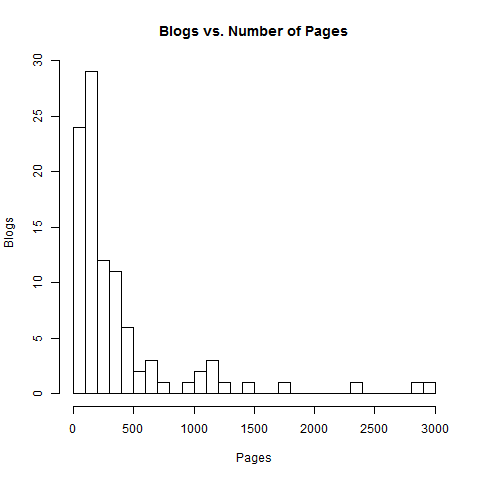
\includegraphics[scale=0.60]{questions/q1/R/q1-histogram1.png}
        \caption{Histogram showing Blogs Vs No of Pages}
        \label{Histogram 1}
    \end{center}
\end{figure}

\newpage

\section{Problem 2}
\label{part2}
Write a Python program that:
\begin{enumerate} 
\item takes one argument, like "Old Dominion" or "Virginia Tech" 
\item takes another argument specified in seconds (e.g., "60" for one minute).
\item takes a URI as a third argument:\\
\url{http://sports.yahoo.com/college-football/scoreboard/}\\
or\\
\url{http://sports.yahoo.com/college-football/scoreboard/?week=2\&conf=all}\\
or\\
\url{ http://sports.yahoo.com/college-football/scoreboard/?week=1\&conf=72}\\
etc.\\
\item dereferences the URI, finds the game corresponding to the team
     argument, prints out the current score (e.g., "Old Dominion 27, 
     East Carolina 17), sleeps for the specified seconds, and then
     repeats (until control-C is hit).
\end{enumerate}

\subsection{Solution}
\begin{enumerate}
\item In order to write this program firstly the source code for the URL should be examined.
\item Find elements in the html code where the team names and scores are located by using "urllib2.urlopen()" function imported from "urllib2" library .check for the div where all the content we want is located and note down the element names
\item Extract the part of code we are looking for by using "BeautifulSoup" library. 
\item The 'div' that had score of a teams are read and stored in to a new array 
\item Get the Team name as a Argument 1 and sleep time as an Argument 2 from a command line argument.
\item Now looping the stored array, check for the desired team name in the array and get the score associated to the team. 
\item By using the sleep method, the program does not exit till the control-C is hit, as the sleep time is given the program keeps updating the result for the given time.
\end{enumerate}

\subsection{Results}
\begin{enumerate}
\item To get the result the below command should be executed 
\begin{verbatim}
retrieve_american_football.py "arizona" 5 \
"http://sports.yahoo.com/college-football/scoreboard/?week=2&conf=all"
\end{verbatim}
\end{enumerate}
\begin{figure}[ht]    
    \begin{center}
        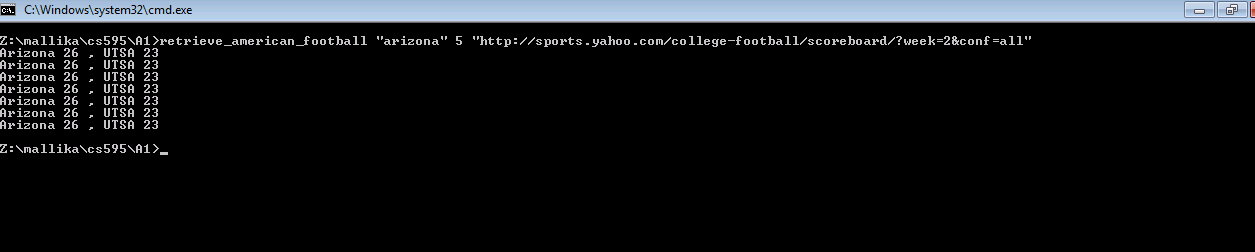
\includegraphics[scale=0.45]{part2-result.png}
        \caption{Sample Output}
        \label{fig:X-distribution}
    \end{center}
\end{figure}

\subsection{Code Listing}
\lstinputlisting[language=Python, breaklines=true]{retrieve_american_football.py}
\section{Problem 3}
\label{part3}
\subsection{Problem 3}
\begin{verbatim}
3.  Now rank the same 10 URIs from question #2, but this time 
by their PageRank.  Use any of the free PR estimaters on the web,
such as:

http://www.prchecker.info/check_page_rank.php
http://www.seocentro.com/tools/search-engines/pagerank.html
http://www.checkpagerank.net/

If you use these tools, you'll have to do so by hand (they have
anti-bot captchas), but there is only 10.  Normalize the values
they give you to be from 0 to 1.0.  Use the same tool on all 10
(again, consistency is more important than accuracy).

Create a table similar to Table 1:

Table 2.  10 hits for the term "shadow", ranked by PageRank.

PageRank	URI
--------	---
0.9		http://bar.com/
0.5		http://foo.com/

Briefly compare and contrast the rankings produced in questions 2
and 3.
\end{verbatim}
\newpage
\subsection{Solution}
\begin{enumerate}
\item Using the URI's acquired form Question 2, I put each into one of the suggested Page Rank Calculators. 
\item Unsurprisingly three websites gave different results for each URI. They seem like they have different data for each sites.We can observe this from Table 1.   
\item So I picked up the values got from PR checker as the Page Ranks for each Website. And I normalized with N/A and Error with 0.0. Table 2 shows the Normalized Ranks for each Website.  
\item Table 3 contains the PageRank and TFIDF values for comparison
\item For this set of URI's, doesn't seem to be a whole lot of correlation between PageRank and TFIDF. 
\item The URI with the highest TFIDF of 0.27 has a PageRank of 0.0 and the page with the lowest TFIDF of 0.02 had a PageRank of 0.7 or 0.0

\end{enumerate}

\newpage
\begin{table}
\small
\begin{tabular}{ | p{2.0cm} | p{2.4cm} | p{2.0cm} | p{8.0cm} | }
\hline
\textbf{Check PageRank} & \textbf{SEO Central} & \textbf{PR Checker} & \textbf{URI} \\
\hline
6/10 & 5/10 & 6/10  & \url{http://www.xxlmag.com } \\
\hline
INVALID DOMAIN & undef & N/A & \url{ http://www.soundclick.com/bands/default.cfm?bandID=1350875} \\
\hline
0/10 & 6/10 & 6/10 & \url{ http://www.bet.com} \\
\hline
INVALID DOMAIN & 2/10 & ERROR & \url{ https://soundcloud.com/scorpios4music} \\
\hline 
5/10 & 5/10 & 5/10 & \url{ http://www.kaskademusic.com/} \\
\hline
3/10 & 3/10 & 3/10 & \url{http://runthetrap.com} \\
\hline
0/10 & undef & N/A & \url{ http://TrueMusicInHipHop.blogspot.com} \\
\hline
5/10 & 5/10 & 5/10 & \url{ http://music.iamlights.com} \\
\hline
0/10 & undef & N/A & \url{ http://www.famoushollywoodbay.com/} \\
\hline
INVALID DOMAIN & 7/10 & 7/10 &\url{ http://www.ew.com/ew/} \\
\hline
\end{tabular}
\caption{PageRank of URIs containing the word \emph{music}, based on the CheckPageRank, SEO Central, and PR Checker Page Rank services}
\label{table:q3-1}
\end{table}

\begin{table}
\small
\begin{tabular}{ | p{2.4cm} | p{8.0cm} | }
\hline
\textbf{PAGE RANK} & \textbf{URI} \\
\hline
0.6  & \url{http://www.xxlmag.com } \\
\hline
0.0 & \url{ http://www.soundclick.com/bands/default.cfm?bandID=1350875} \\
\hline
0.6 & \url{ http://www.bet.com} \\
\hline
0.0 & \url{ https://soundcloud.com/scorpios4music} \\
\hline 
0.5 & \url{ http://www.kaskademusic.com/} \\
\hline
0.3 & \url{http://runthetrap.com} \\
\hline
0.0 & \url{ http://TrueMusicInHipHop.blogspot.com} \\
\hline
0.5 & \url{ http://music.iamlights.com} \\
\hline
0.0 & \url{ http://www.famoushollywoodbay.com/} \\
\hline
0.7 &\url{ http://www.ew.com/ew/} \\
\hline
\end{tabular}
\caption{Normalized PageRank of URIs containing the word \emph{music}, based on the PR Checker Page Rank services}
\label{table:q3-2}
\end{table}
\begin{table}
\small
\begin{tabular}{ | p{2.4cm} | p{2.4cm} | p{8.0cm} | }
\hline
\textbf{TFIDF} & \textbf{PAGE RANK} & \textbf{URI}  \\
\hline
0.02 & 0.7 &\url{ http://www.ew.com/ew/} \\
\hline
0.07 & 0.6  & \url{http://www.xxlmag.com } \\
\hline
0.07 & 0.6 & \url{ http://www.bet.com} \\
\hline
0.11 & 0.5 & \url{ http://www.kaskademusic.com/} \\
\hline
0.06 & 0.5 & \url{ http://music.iamlights.com} \\
\hline
0.04 & 0.3 & \url{http://runthetrap.com} \\
\hline
0.02 & 0.0 & \url{ http://www.soundclick.com/bands/default.cfm?bandID=1350875} \\
\hline
0.27 & 0.0 & \url{ https://soundcloud.com/scorpios4music} \\
\hline 
0.10 & 0.0 & \url{ http://TrueMusicInHipHop.blogspot.com} \\
\hline
0.04 & 0.0 & \url{ http://www.famoushollywoodbay.com/} \\


\hline
\end{tabular}
\caption{PageRank of URIs containing the word \emph{football}, based on the PR Checker Page Rank service, with \emph{Not available} replaced with $0$ and all other values normalized, sorted by decreasing PageRank}
\label{table:q3-3}
\end{table}
\section{Problem 4}
\label{part4}
\subsection*{Question}
\begingroup
\begin{verbatim}
Use MDS to create a JPEG of the blogs similar to slide 29.  
How many iterations were required?
\end{verbatim}
\subsection{Answer}
\begin{enumerate}
\item The blog space is generated using multidimensional scaling from the script \verb+makeMDS.py+ shown in Listing \ref{lst:mds-code}, which makes use of Toby Segaran's \emph{clusters.py} using the functions \emph{scaledown} on line $7$ and \emph{draw2d} on line $9$.


\lstinputlisting[language=python, frame=single,breaklines=true, caption={Python script for generating a MDS from the blog data},captionpos=b, numbers=left, showspaces=false,label=lst:mds-code, showstringspaces=false, basicstyle=\footnotesize]{questions/q4/makeMDS.py}

\item unfortunately the blog space produced does not fit well on a letter-sized page shown in Figure \ref{fig:q4MDS}.
\item Listing \ref{lst:q4output} shows the output from running this script, which took $253$ iterations on this run.
\end{enumerate}
\newpage
\begin{figure}[h]
\centerline{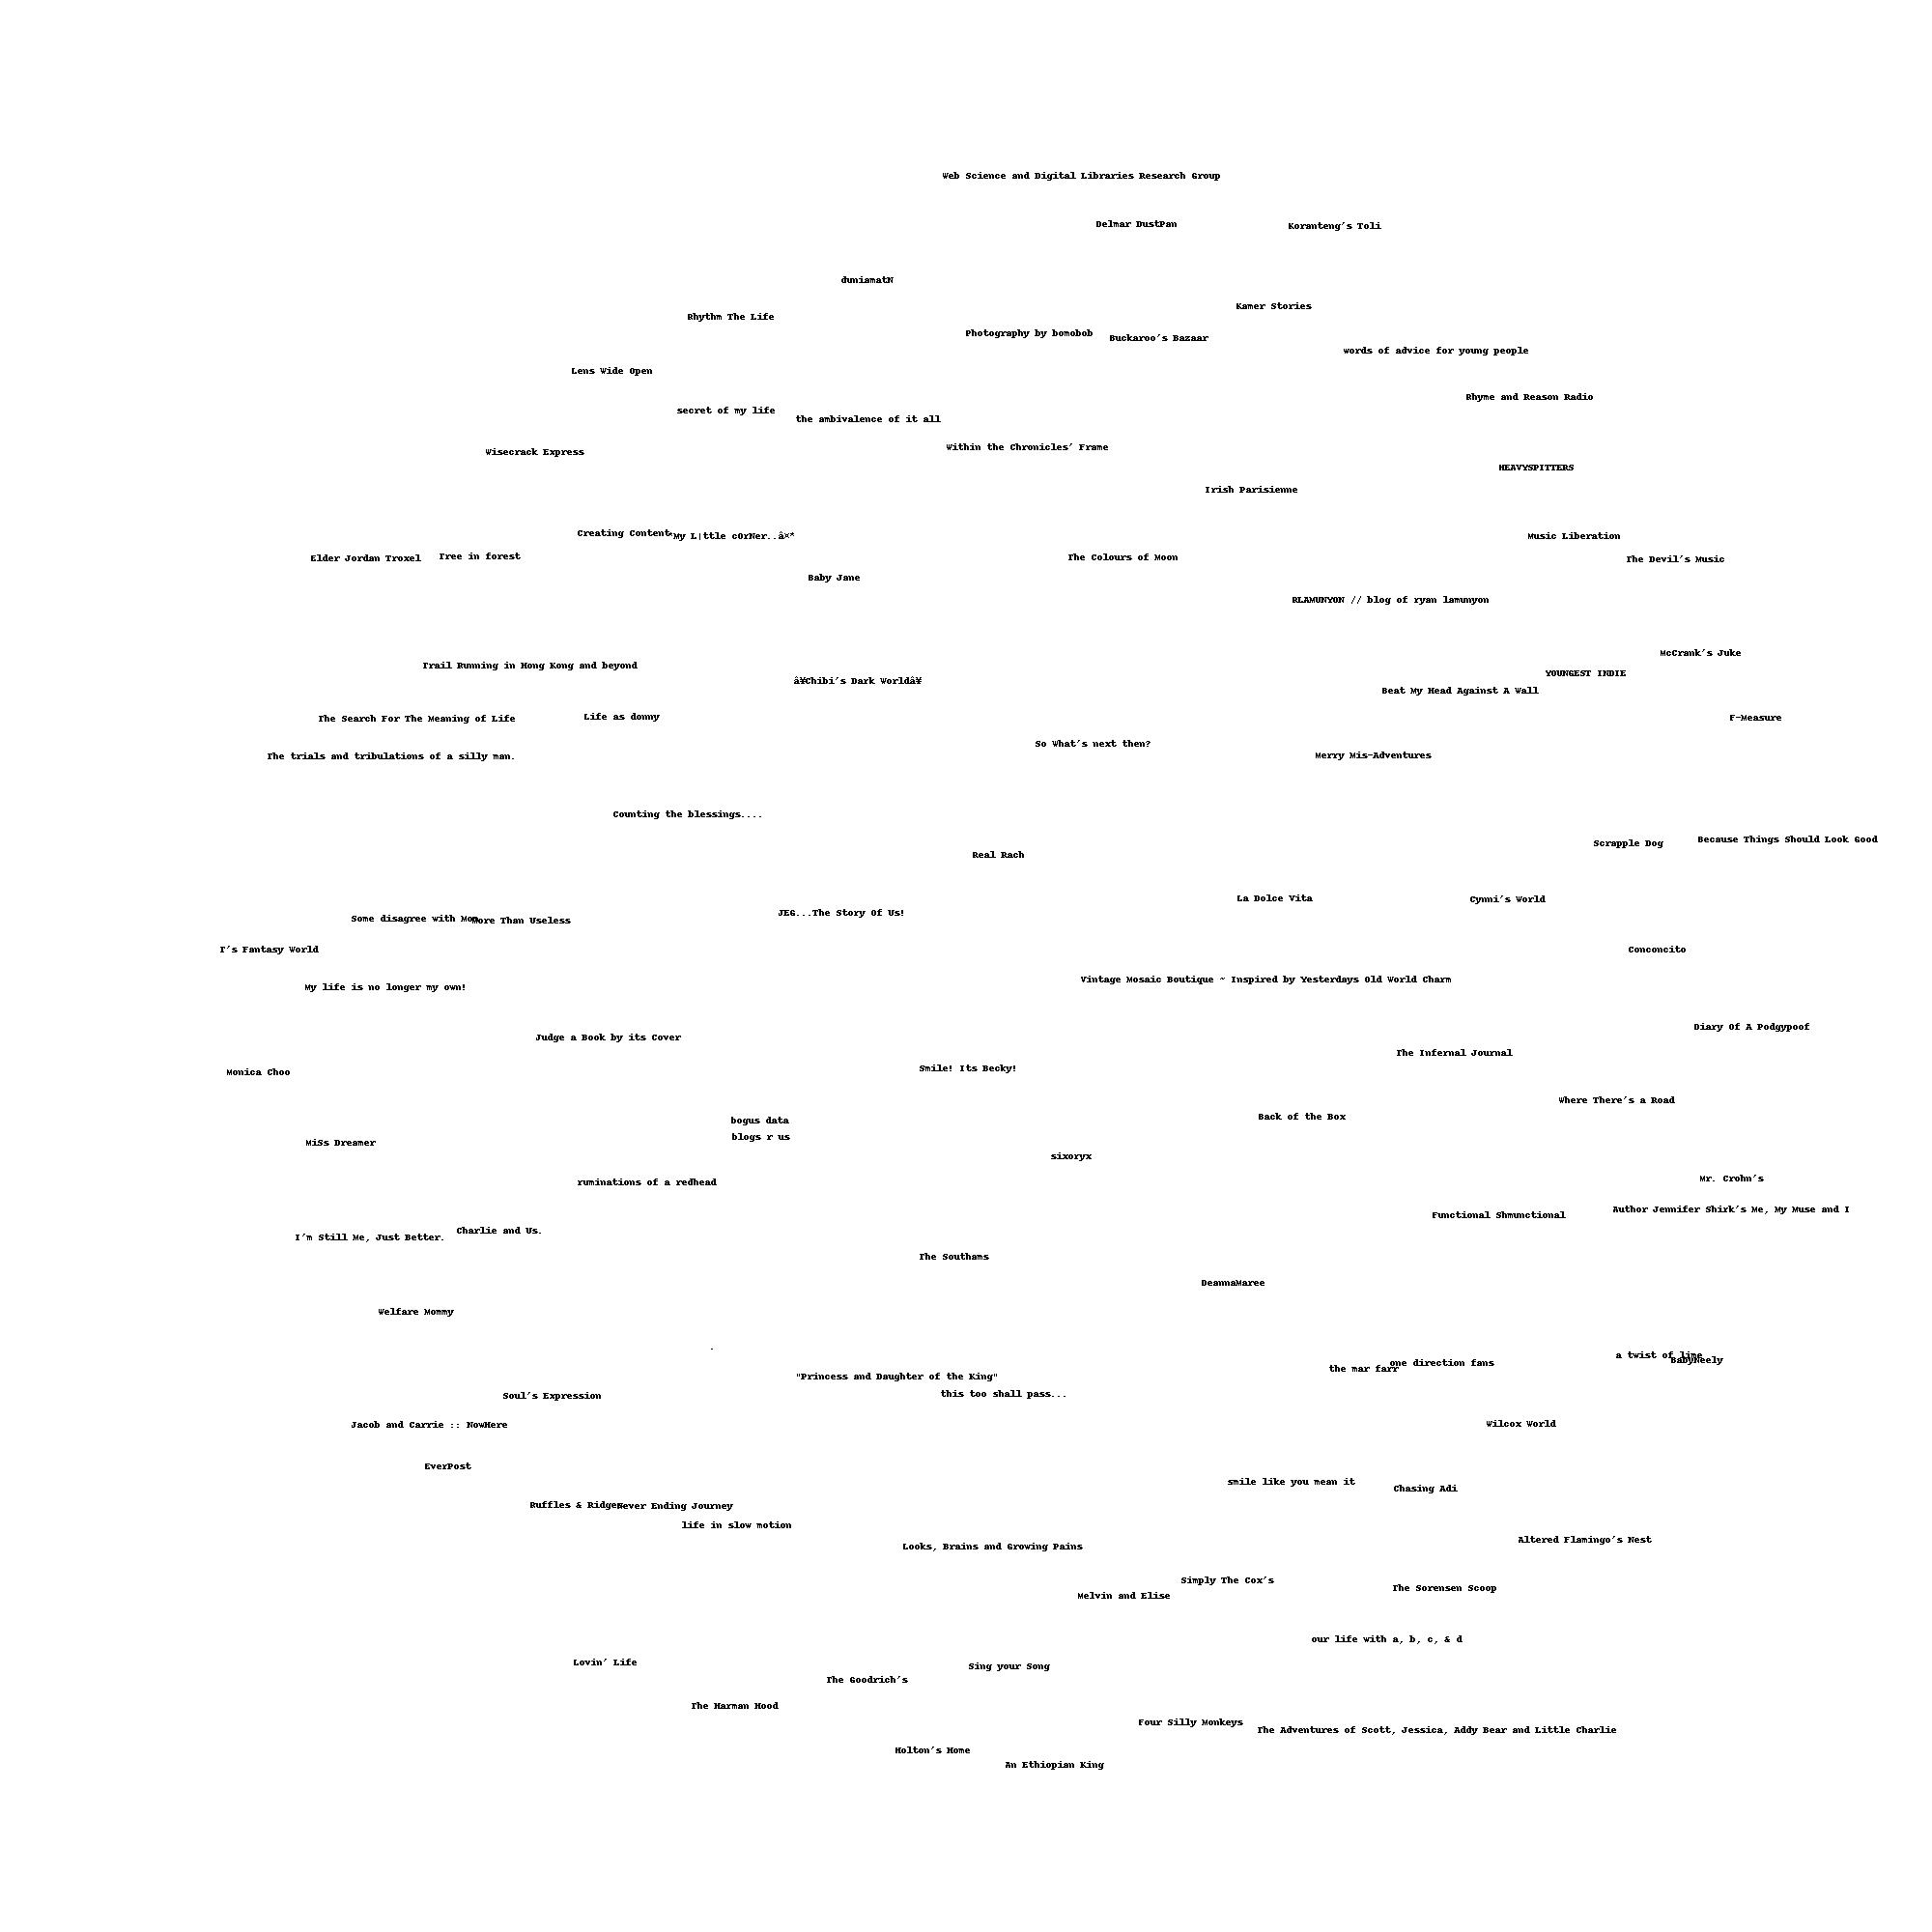
\includegraphics[scale=0.26]{questions/q4/blogs2d.jpg}}
\caption{Blog space produced by the \emph{makeMDS.py} script}
\label{fig:q4MDS}
\end{figure}

\lstinputlisting[frame=single,caption={Output from script \emph{makeMDS.py}},label=lst:q4output,captionpos=b,numbers=left,showspaces=false,showstringspaces=false,basicstyle=\footnotesize]{questions/q4/q5-mds.txt}
\newpage


\bibliographystyle{plain}
\bibliography{a4}
\nocite{*}


\end{document}

